
% DISSECTION

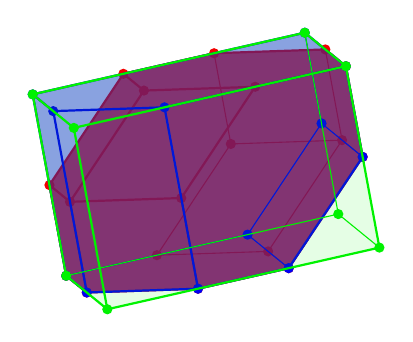
\begin{tikzpicture}%
  [x={(0.217568cm, -0.177363cm)},
  y={(0.959795cm, 0.217568cm)},
  z={(-0.177363cm, 0.959795cm)},
  scale=.6,
  zono/.style={color=red!95!black},
  acco/.style={color=blue!95!black},
  para/.style={color=green!95!black},
  back/.style={thin},
  edge/.style={thick},
  facet/.style={fill opacity=0.6},
  facetzono/.style={fill opacity=0.8},
  facetacco/.style={fill opacity=0.4},
  facetpara/.style={fill opacity=0.1},
  vertex/.style={inner sep=1pt,circle,draw=green!25!black,fill=green!75!black,thick,anchor=base}]

%% ZONO
%% Coordinate of the vertices:
\coordinate (-2.00000, -3.00000, -2.00000) at (-2.00000, -3.00000, -2.00000);
\coordinate (-2.00000, -3.00000, 0.00000) at (-2.00000, -3.00000, 0.00000);
\coordinate (-2.00000, -1.00000, -2.00000) at (-2.00000, -1.00000, -2.00000);
\coordinate (-2.00000, -1.00000, 2.00000) at (-2.00000, -1.00000, 2.00000);
\coordinate (-2.00000, 1.00000, 0.00000) at (-2.00000, 1.00000, 0.00000);
\coordinate (-2.00000, 1.00000, 2.00000) at (-2.00000, 1.00000, 2.00000);
\coordinate (2.00000, 3.00000, 2.00000) at (2.00000, 3.00000, 2.00000);
\coordinate (2.00000, 3.00000, 0.00000) at (2.00000, 3.00000, 0.00000);
\coordinate (2.00000, 1.00000, 2.00000) at (2.00000, 1.00000, 2.00000);
\coordinate (2.00000, 1.00000, -2.00000) at (2.00000, 1.00000, -2.00000);
\coordinate (2.00000, -1.00000, 0.00000) at (2.00000, -1.00000, 0.00000);
\coordinate (2.00000, -1.00000, -2.00000) at (2.00000, -1.00000, -2.00000);
\coordinate (0.00000, -3.00000, -2.00000) at (0.00000, -3.00000, -2.00000);
\coordinate (0.00000, -3.00000, 0.00000) at (0.00000, -3.00000, 0.00000);
\coordinate (0.00000, -1.00000, 2.00000) at (0.00000, -1.00000, 2.00000);
\coordinate (0.00000, 1.00000, -2.00000) at (0.00000, 1.00000, -2.00000);
\coordinate (0.00000, 3.00000, 0.00000) at (0.00000, 3.00000, 0.00000);
\coordinate (0.00000, 3.00000, 2.00000) at (0.00000, 3.00000, 2.00000);

%% Drawing edges in the back
\draw[edge,back,zono] (-2.00000, -3.00000, -2.00000) -- (-2.00000, -1.00000, -2.00000);
\draw[edge,back,zono] (-2.00000, -1.00000, -2.00000) -- (-2.00000, 1.00000, 0.00000);
\draw[edge,back,zono] (-2.00000, -1.00000, -2.00000) -- (0.00000, 1.00000, -2.00000);
\draw[edge,back,zono] (-2.00000, 1.00000, 0.00000) -- (-2.00000, 1.00000, 2.00000);
\draw[edge,back,zono] (-2.00000, 1.00000, 0.00000) -- (0.00000, 3.00000, 0.00000);
\draw[edge,back,zono] (2.00000, 3.00000, 0.00000) -- (0.00000, 3.00000, 0.00000);
\draw[edge,back,zono] (2.00000, 1.00000, -2.00000) -- (0.00000, 1.00000, -2.00000);
\draw[edge,back,zono] (0.00000, 1.00000, -2.00000) -- (0.00000, 3.00000, 0.00000);
\draw[edge,back,zono] (0.00000, 3.00000, 0.00000) -- (0.00000, 3.00000, 2.00000);

%% Drawing vertices in the back
\node[vertex,zono] at (0.00000, 3.00000, 0.00000)     {};
\node[vertex,zono] at (-2.00000, -1.00000, -2.00000)     {};
\node[vertex,zono] at (-2.00000, 1.00000, 0.00000)     {};
\node[vertex,zono] at (0.00000, 1.00000, -2.00000)     {};

%% Drawing the facets
\fill[facetzono,zono] (2.00000, -1.00000, -2.00000) -- (2.00000, 1.00000, -2.00000) -- (2.00000, 3.00000, 0.00000) -- (2.00000, 3.00000, 2.00000) -- (2.00000, 1.00000, 2.00000) -- (2.00000, -1.00000, 0.00000) -- cycle {};
\fill[facetzono,zono] (2.00000, 1.00000, 2.00000) -- (2.00000, 3.00000, 2.00000) -- (0.00000, 3.00000, 2.00000) -- (-2.00000, 1.00000, 2.00000) -- (-2.00000, -1.00000, 2.00000) -- (0.00000, -1.00000, 2.00000) -- cycle {};
\fill[facetzono,zono] (0.00000, -1.00000, 2.00000) -- (-2.00000, -1.00000, 2.00000) -- (-2.00000, -3.00000, 0.00000) -- (0.00000, -3.00000, 0.00000) -- cycle {};
\fill[facetzono,zono] (0.00000, -3.00000, 0.00000) -- (-2.00000, -3.00000, 0.00000) -- (-2.00000, -3.00000, -2.00000) -- (0.00000, -3.00000, -2.00000) -- cycle {};
\fill[facetzono,zono] (0.00000, -3.00000, 0.00000) -- (2.00000, -1.00000, 0.00000) -- (2.00000, -1.00000, -2.00000) -- (0.00000, -3.00000, -2.00000) -- cycle {};
\fill[facetzono,zono] (0.00000, -1.00000, 2.00000) -- (2.00000, 1.00000, 2.00000) -- (2.00000, -1.00000, 0.00000) -- (0.00000, -3.00000, 0.00000) -- cycle {};

%% Drawing edges in the front
\draw[edge,zono] (-2.00000, -3.00000, -2.00000) -- (-2.00000, -3.00000, 0.00000);
\draw[edge,zono] (-2.00000, -3.00000, -2.00000) -- (0.00000, -3.00000, -2.00000);
\draw[edge,zono] (-2.00000, -3.00000, 0.00000) -- (-2.00000, -1.00000, 2.00000);
\draw[edge,zono] (-2.00000, -3.00000, 0.00000) -- (0.00000, -3.00000, 0.00000);
\draw[edge,zono] (-2.00000, -1.00000, 2.00000) -- (-2.00000, 1.00000, 2.00000);
\draw[edge,zono] (-2.00000, -1.00000, 2.00000) -- (0.00000, -1.00000, 2.00000);
\draw[edge,zono] (-2.00000, 1.00000, 2.00000) -- (0.00000, 3.00000, 2.00000);
\draw[edge,zono] (2.00000, 3.00000, 2.00000) -- (2.00000, 3.00000, 0.00000);
\draw[edge,zono] (2.00000, 3.00000, 2.00000) -- (2.00000, 1.00000, 2.00000);
\draw[edge,zono] (2.00000, 3.00000, 2.00000) -- (0.00000, 3.00000, 2.00000);
\draw[edge,zono] (2.00000, 3.00000, 0.00000) -- (2.00000, 1.00000, -2.00000);
\draw[edge,zono] (2.00000, 1.00000, 2.00000) -- (2.00000, -1.00000, 0.00000);
\draw[edge,zono] (2.00000, 1.00000, 2.00000) -- (0.00000, -1.00000, 2.00000);
\draw[edge,zono] (2.00000, 1.00000, -2.00000) -- (2.00000, -1.00000, -2.00000);
\draw[edge,zono] (2.00000, -1.00000, 0.00000) -- (2.00000, -1.00000, -2.00000);
\draw[edge,zono] (2.00000, -1.00000, 0.00000) -- (0.00000, -3.00000, 0.00000);
\draw[edge,zono] (2.00000, -1.00000, -2.00000) -- (0.00000, -3.00000, -2.00000);
\draw[edge,zono] (0.00000, -3.00000, -2.00000) -- (0.00000, -3.00000, 0.00000);
\draw[edge,zono] (0.00000, -3.00000, 0.00000) -- (0.00000, -1.00000, 2.00000);

%% Drawing the vertices in the front
\node[vertex,zono] at (-2.00000, -3.00000, -2.00000)     {};
\node[vertex,zono] at (-2.00000, -3.00000, 0.00000)     {};
\node[vertex,zono] at (-2.00000, -1.00000, 2.00000)     {};
\node[vertex,zono] at (-2.00000, 1.00000, 2.00000)     {};
\node[vertex,zono] at (2.00000, 3.00000, 2.00000)     {};
\node[vertex,zono] at (2.00000, 3.00000, 0.00000)     {};
\node[vertex,zono] at (2.00000, 1.00000, 2.00000)     {};
\node[vertex,zono] at (2.00000, 1.00000, -2.00000)     {};
\node[vertex,zono] at (2.00000, -1.00000, 0.00000)     {};
\node[vertex,zono] at (2.00000, -1.00000, -2.00000)     {};
\node[vertex,zono] at (0.00000, -3.00000, -2.00000)     {};
\node[vertex,zono] at (0.00000, -3.00000, 0.00000)     {};
\node[vertex,zono] at (0.00000, -1.00000, 2.00000)     {};
\node[vertex,zono] at (0.00000, 3.00000, 2.00000)     {};

%% ACCO
%% Coordinate of the vertices:
\coordinate (0.00000, -3.00000, -2.00000) at (0.00000, -3.00000, -2.00000);
\coordinate (2.00000, -1.00000, -2.00000) at (2.00000, -1.00000, -2.00000);
\coordinate (2.00000, -1.00000, 2.00000) at (2.00000, -1.00000, 2.00000);
\coordinate (2.00000, 3.00000, 2.00000) at (2.00000, 3.00000, 2.00000);
\coordinate (2.00000, 3.00000, 0.00000) at (2.00000, 3.00000, 0.00000);
\coordinate (2.00000, 1.00000, -2.00000) at (2.00000, 1.00000, -2.00000);
\coordinate (0.00000, -3.00000, 2.00000) at (0.00000, -3.00000, 2.00000);
\coordinate (-2.00000, -3.00000, 2.00000) at (-2.00000, -3.00000, 2.00000);
\coordinate (-2.00000, -3.00000, -2.00000) at (-2.00000, -3.00000, -2.00000);
\coordinate (-2.00000, 3.00000, 2.00000) at (-2.00000, 3.00000, 2.00000);
\coordinate (-2.00000, 3.00000, 0.00000) at (-2.00000, 3.00000, 0.00000);
\coordinate (-2.00000, 1.00000, -2.00000) at (-2.00000, 1.00000, -2.00000);

%% Drawing edges in the back
\draw[edge,back,acco] (2.00000, 3.00000, 0.00000) -- (-2.00000, 3.00000, 0.00000);
\draw[edge,back,acco] (2.00000, 1.00000, -2.00000) -- (-2.00000, 1.00000, -2.00000);
\draw[edge,back,acco] (-2.00000, -3.00000, -2.00000) -- (-2.00000, 1.00000, -2.00000);
\draw[edge,back,acco] (-2.00000, 3.00000, 2.00000) -- (-2.00000, 3.00000, 0.00000);
\draw[edge,back,acco] (-2.00000, 3.00000, 0.00000) -- (-2.00000, 1.00000, -2.00000);

%% Drawing vertices in the back
\node[vertex,acco] at (-2.00000, 3.00000, 0.00000)     {};
\node[vertex,acco] at (-2.00000, 1.00000, -2.00000)     {};

%% Drawing the facets
\fill[facetacco,acco] (2.00000, 1.00000, -2.00000) -- (2.00000, -1.00000, -2.00000) -- (2.00000, -1.00000, 2.00000) -- (2.00000, 3.00000, 2.00000) -- (2.00000, 3.00000, 0.00000) -- cycle {};
\fill[facetacco,acco] (0.00000, -3.00000, 2.00000) -- (0.00000, -3.00000, -2.00000) -- (2.00000, -1.00000, -2.00000) -- (2.00000, -1.00000, 2.00000) -- cycle {};
\fill[facetacco,acco] (-2.00000, 3.00000, 2.00000) -- (2.00000, 3.00000, 2.00000) -- (2.00000, -1.00000, 2.00000) -- (0.00000, -3.00000, 2.00000) -- (-2.00000, -3.00000, 2.00000) -- cycle {};
\fill[facetacco,acco] (-2.00000, -3.00000, -2.00000) -- (0.00000, -3.00000, -2.00000) -- (0.00000, -3.00000, 2.00000) -- (-2.00000, -3.00000, 2.00000) -- cycle {};

%% Drawing edges in the front
\draw[edge,acco] (0.00000, -3.00000, -2.00000) -- (2.00000, -1.00000, -2.00000);
\draw[edge,acco] (0.00000, -3.00000, -2.00000) -- (0.00000, -3.00000, 2.00000);
\draw[edge,acco] (0.00000, -3.00000, -2.00000) -- (-2.00000, -3.00000, -2.00000);
\draw[edge,acco] (2.00000, -1.00000, -2.00000) -- (2.00000, -1.00000, 2.00000);
\draw[edge,acco] (2.00000, -1.00000, -2.00000) -- (2.00000, 1.00000, -2.00000);
\draw[edge,acco] (2.00000, -1.00000, 2.00000) -- (2.00000, 3.00000, 2.00000);
\draw[edge,acco] (2.00000, -1.00000, 2.00000) -- (0.00000, -3.00000, 2.00000);
\draw[edge,acco] (2.00000, 3.00000, 2.00000) -- (2.00000, 3.00000, 0.00000);
\draw[edge,acco] (2.00000, 3.00000, 2.00000) -- (-2.00000, 3.00000, 2.00000);
\draw[edge,acco] (2.00000, 3.00000, 0.00000) -- (2.00000, 1.00000, -2.00000);
\draw[edge,acco] (0.00000, -3.00000, 2.00000) -- (-2.00000, -3.00000, 2.00000);
\draw[edge,acco] (-2.00000, -3.00000, 2.00000) -- (-2.00000, -3.00000, -2.00000);
\draw[edge,acco] (-2.00000, -3.00000, 2.00000) -- (-2.00000, 3.00000, 2.00000);

%% Drawing the vertices in the front
\node[vertex,acco] at (0.00000, -3.00000, -2.00000)     {};
\node[vertex,acco] at (2.00000, -1.00000, -2.00000)     {};
\node[vertex,acco] at (2.00000, -1.00000, 2.00000)     {};
\node[vertex,acco] at (2.00000, 3.00000, 2.00000)     {};
\node[vertex,acco] at (2.00000, 3.00000, 0.00000)     {};
\node[vertex,acco] at (2.00000, 1.00000, -2.00000)     {};
\node[vertex,acco] at (0.00000, -3.00000, 2.00000)     {};
\node[vertex,acco] at (-2.00000, -3.00000, 2.00000)     {};
\node[vertex,acco] at (-2.00000, -3.00000, -2.00000)     {};
\node[vertex,acco] at (-2.00000, 3.00000, 2.00000)     {};

%% PARA
%% Coordinate of the vertices:
\coordinate (2.00000, -3.00000, -2.00000) at (2.00000, -3.00000, -2.00000);
\coordinate (2.00000, 3.00000, -2.00000) at (2.00000, 3.00000, -2.00000);
\coordinate (2.00000, 3.00000, 2.00000) at (2.00000, 3.00000, 2.00000);
\coordinate (2.00000, -3.00000, 2.00000) at (2.00000, -3.00000, 2.00000);
\coordinate (-2.00000, -3.00000, 2.00000) at (-2.00000, -3.00000, 2.00000);
\coordinate (-2.00000, -3.00000, -2.00000) at (-2.00000, -3.00000, -2.00000);
\coordinate (-2.00000, 3.00000, -2.00000) at (-2.00000, 3.00000, -2.00000);
\coordinate (-2.00000, 3.00000, 2.00000) at (-2.00000, 3.00000, 2.00000);

%% Drawing edges in the back
\draw[edge,back,para] (2.00000, 3.00000, -2.00000) -- (-2.00000, 3.00000, -2.00000);
\draw[edge,back,para] (-2.00000, -3.00000, -2.00000) -- (-2.00000, 3.00000, -2.00000);
\draw[edge,back,para] (-2.00000, 3.00000, -2.00000) -- (-2.00000, 3.00000, 2.00000);

%% Drawing vertices in the back
\node[vertex,para] at (-2.00000, 3.00000, -2.00000)     {};

%% Drawing the facets
\fill[facetpara,para] (2.00000, -3.00000, 2.00000) -- (2.00000, -3.00000, -2.00000) -- (2.00000, 3.00000, -2.00000) -- (2.00000, 3.00000, 2.00000) -- cycle {};
\fill[facetpara,para] (-2.00000, 3.00000, 2.00000) -- (2.00000, 3.00000, 2.00000) -- (2.00000, -3.00000, 2.00000) -- (-2.00000, -3.00000, 2.00000) -- cycle {};
\fill[facetpara,para] (-2.00000, -3.00000, -2.00000) -- (2.00000, -3.00000, -2.00000) -- (2.00000, -3.00000, 2.00000) -- (-2.00000, -3.00000, 2.00000) -- cycle {};

%% Drawing edges in the front
\draw[edge,para] (2.00000, -3.00000, -2.00000) -- (2.00000, 3.00000, -2.00000);
\draw[edge,para] (2.00000, -3.00000, -2.00000) -- (2.00000, -3.00000, 2.00000);
\draw[edge,para] (2.00000, -3.00000, -2.00000) -- (-2.00000, -3.00000, -2.00000);
\draw[edge,para] (2.00000, 3.00000, -2.00000) -- (2.00000, 3.00000, 2.00000);
\draw[edge,para] (2.00000, 3.00000, 2.00000) -- (2.00000, -3.00000, 2.00000);
\draw[edge,para] (2.00000, 3.00000, 2.00000) -- (-2.00000, 3.00000, 2.00000);
\draw[edge,para] (2.00000, -3.00000, 2.00000) -- (-2.00000, -3.00000, 2.00000);
\draw[edge,para] (-2.00000, -3.00000, 2.00000) -- (-2.00000, -3.00000, -2.00000);
\draw[edge,para] (-2.00000, -3.00000, 2.00000) -- (-2.00000, 3.00000, 2.00000);

%% Drawing the vertices in the front
\node[vertex,para] at (2.00000, -3.00000, -2.00000)     {};
\node[vertex,para] at (2.00000, 3.00000, -2.00000)     {};
\node[vertex,para] at (2.00000, 3.00000, 2.00000)     {};
\node[vertex,para] at (2.00000, -3.00000, 2.00000)     {};
\node[vertex,para] at (-2.00000, -3.00000, 2.00000)     {};
\node[vertex,para] at (-2.00000, -3.00000, -2.00000)     {};
\node[vertex,para] at (-2.00000, 3.00000, 2.00000)     {};

\end{tikzpicture}